\documentclass[]{article}
\usepackage{abstract}
\usepackage[dvipdfmx]{graphicx}


\title{Modeling Autonomous Vehicles at an Intersection without a Traffic Light}
\author{Yui Sahara*  Mazaki Nakamura* 	*Nakamura Lab.}
\date{}
\begin{document}
\maketitle
\begin{abstract}
	Automatic driving technology has been in rapid development.  For safe and efficient cities with a lot of such autonomous vehicles, we need to consider not only control systems for individual vehicles but also those for a group of vehicles.  In this article, we investigate a way to model and verify of autonomous-vehicle at intersection without traffic light using a model checking technique.
\end{abstract}

\section{Introduction}
	  Automatic driving technology is in rapid development.  Automatic driving is divided into five levels depending on the technology installed.  In Japan, general cars install level 2 supporting driver.  In the future,  Japan government will set a goal that the vehicles installed level 4 become popular.  If a lot of automatic driving cars are used in a city, some problems may occur.  Thus, we need autonomous-vehicle group control algorithms.  In this paper, we verify the autonomous-vehicle group control algorithms with formal method.
\section{Past research}
	Autonomous-vehicle systems support drivers to avoid conflict and to control safety.  Cars are necessary for our lifestyles, but traffic accidents happen anytime.  Therefore, we ought not drive car.  Autonomous-vehicle is necessary for human life in the future.  A collision avoidance systems were developed to protect drivers. 
\section{Methods}
	\subsection{Model checking tool UPPAAL}
		UPPAAL \cite{u1} is an integrated tool environment for modeling, simulation, and verification of real-time systems.  UPPAAL provides graphical interface to describe timed automata and simulate and verify them. UPPAAL's timed automata is an extension of usual timed automata.  We declare local and global variables for data types and clocks. In UPPAAL, a system model consists of collection of timed automata.  Global variables are declared for a system model. Timed automata \cite{u2} consist of a finite number of clock variables, a finite number of locations, and transitions between locations.  A clock variable stores time progress of continuous state of the system.
	\subsection{Model of Intersection}
		An intersection without a traffic light is one lane on one side(Fig.\ref{Intersec}).  Cars that turn left can pass at the same time in this intersection.  
		\begin{figure}
		\centering
		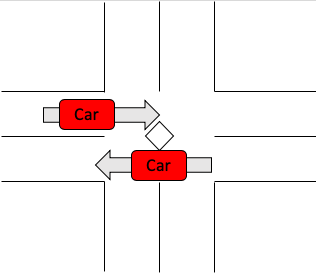
\includegraphics[width=60mm]{model_Inter.png}
		\caption{Model of Intersection without Traffic Lights}
		\label{Intersec}
		\end{figure}
\section{Results}
	\subsection{Timed Automaton of A Intersection}
		In this section we give a system model of intersections with several autonomous vehicles.  There is a timed automata of intersection without traffic lights using UPPAAL(Fig.\ref{temp}).  This is template of timed automata.  Parameters are declared direction of cars, cars' start points, and cars' end points.  Global declarations and local declarations are shown Fig.\ref{GD} and Fig.\ref{LD}.  Moreover, we declare systems instance(Fig.\ref{SysD}). System declarations make timed automata from template.
		\begin{figure}
		\centering
		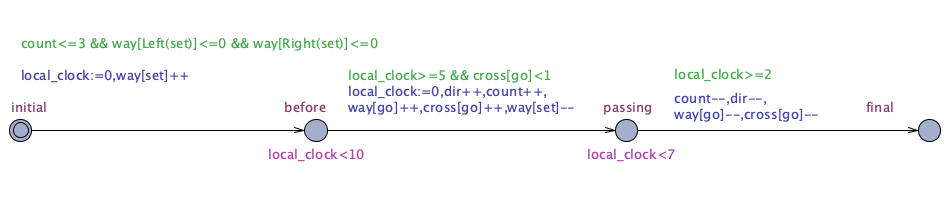
\includegraphics[width=100mm]{temp.png}
		\caption{Template of Timed Automata}
		\label{temp}
		\end{figure}
		
		\begin{figure}
		\centering
		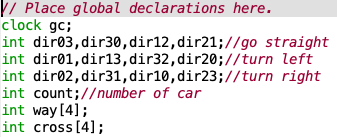
\includegraphics[width=80mm]{Global_dec.png}
		\caption{Global declarations}
		\label{GD}
		\end{figure}
		\begin{figure}
		\centering
		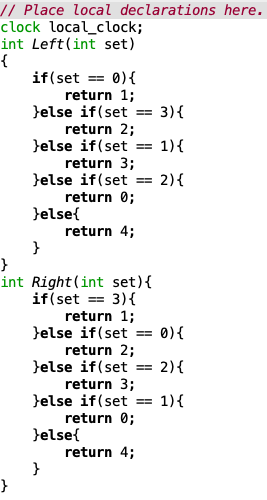
\includegraphics[width=70mm]{local_dec.png}
		\caption{Local declarations}
		\label{LD}
		\end{figure}
		\begin{figure}
		\centering
		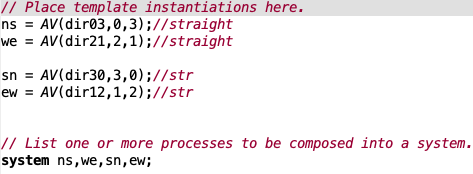
\includegraphics[width=100mm]{SysD.png}
		\caption{System declarations}
		\label{SysD}
		\end{figure}
	\subsection{Verification}
		A car takes from seven units time to seventeen units time to pass the intersection. In this section, we verify the shortest time of four cars' passing an intersection.  Verification uses like next formula. First formula verify reachability, second formula verify minimality.  Verification results that shortest time is 14 units time.
		\[
		E<> (gc == 14 and ns.final and sn.final and ew.final and we.final)
		\]
		\[
		A [ ] (gc < 14 imply not (ns.final and sn.final and ew.final and we.final))
		\]
\section{Conclusion}
	We proposed a modeling and verification method of autonomous-vehicle group control algorithms using UPPAAL. We could verify and modeling the behavior of autonomous vehicles at an intersection.
\section*{Biographical Statement}
Yui Sahara is graduate student in Nakamura Laboratory at Toyama Prefectural University in the Graduate School Engineering majoring Information Systems Engineering.  She received Bachelor of Engineering from Toyama Prefectural University at 2019.  Her recent work includes "Modeling and verification of autonomous-vehicle group control algorithms using UPPAAL"(ISCIE, May, 2019).  She is researching performance model verification of autonomous-vehicle group control algorithms using a model checking technique.
\begin{thebibliography}{2}
 \bibitem{u1}{Kim Guldstrand Larsen and Paul Pettersson and Wang Yi, UPPAAL in a Nutshell, International Jour- nal of Software Tools for Technology Transfer, Vol.1, No.1-2, pp.134-152, 1997.}
 \bibitem{u2}{Timed Automata: Semantics, Algorithms and Tools, Johan Bengtsson and Wang Yi. In Lecture Notes on Concurrency and Petri Nets. W. Reisig and G. Rozenberg (eds.), LNCS 3098, Springer-Verlag, 2004.}
\end{thebibliography}
\end{document}